\section{Model 1}

The results displayed in this section are for the
%uncertainty involved in the calculation of flamespeed depending only on one
%parameter i.e
of the activation energy for the fall off reaction in the ozone
mechanism. The percentage of ozone is taken as 40, 46, 53, 75 and 100
percent acccording to the experimental data
available~\cite{Streng}. The results are displayed in five
sections. In the
first section, the plots are shown for raw chain size, histogram, and CDF
for parameter $E_3$. In the second section, for
constant surrogate size, the number of samples are changed from 1e5 to
1e7 and convergence is observed. In the third part of the results,
convergence study is done for surrogates with differing number of
interpolation points. In the
fourth section, we ensure that samples of the parameter from which we are
drawing are fitting the flamespeed values of the experiment. Also for
varying size the map point of the resulting pdf does not change
greatly. In the fifth section mean and correlation plots are shown for
the samples of the parameter. The surrogates for individual
concentrations are constructed using linear interpolation
function. The initial guess for the map point is calculated using
nelder mead optimization technique. After supplying initial guess over
large domain it is found that the map point is the same no matter
where we start our guess.

\subsection{ Statistics }

 In this section, we display results for sample size 1e7 and surrogate
 of 1000 points. We show the raw samples generated by MCMC and plot
 the histogram for the same. Later we plot the kde and cdf. The last
 plot shows the log of the likelihood function. We can clearly see the
 burning period for the samples.

\begin{figure}[H]
\subfloat[MCMC raw chain of samples \label{subfig-1:Raw Chain}]{%
     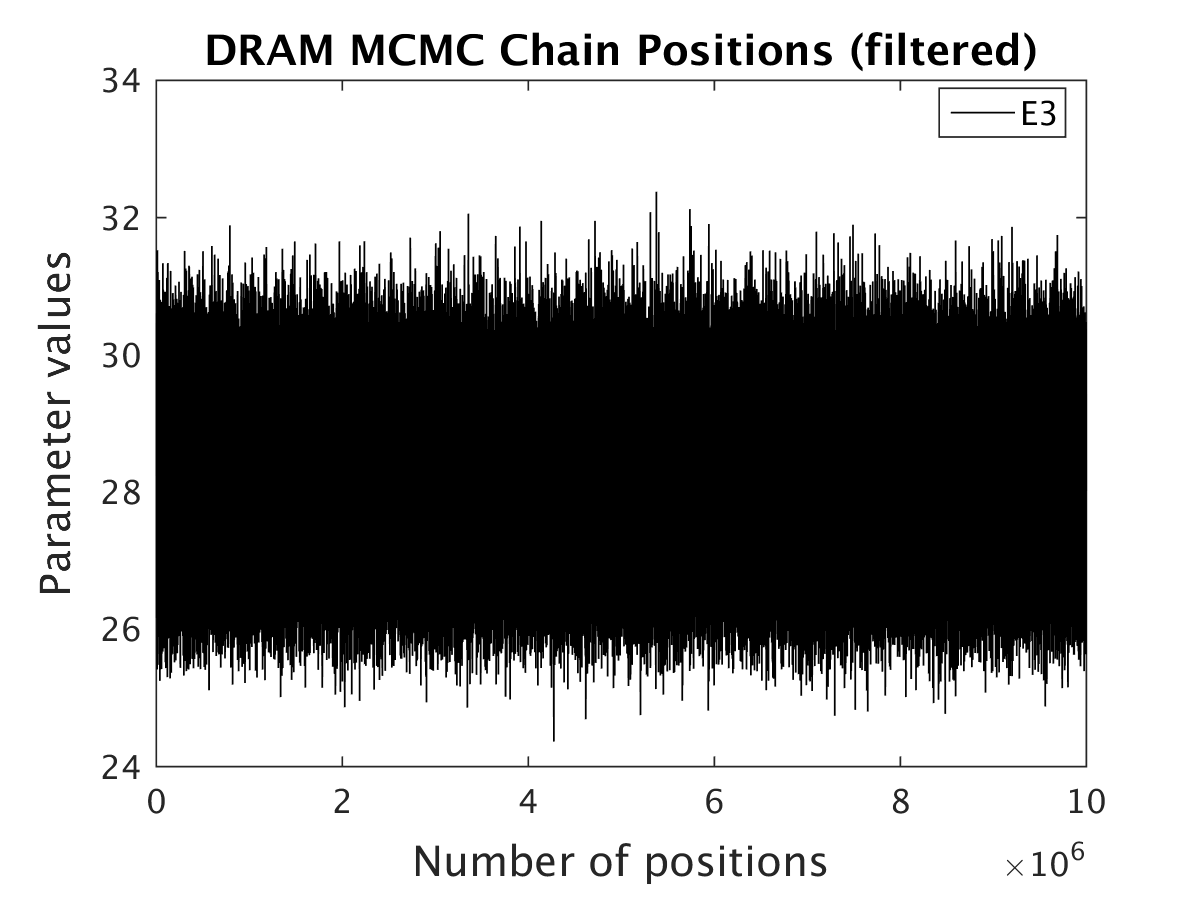
\includegraphics[scale=0.45]{model_1/simple_ip_chain_pos_filt}
    }
\subfloat[Histogram\label{subfig-2:Histogram}]{%
     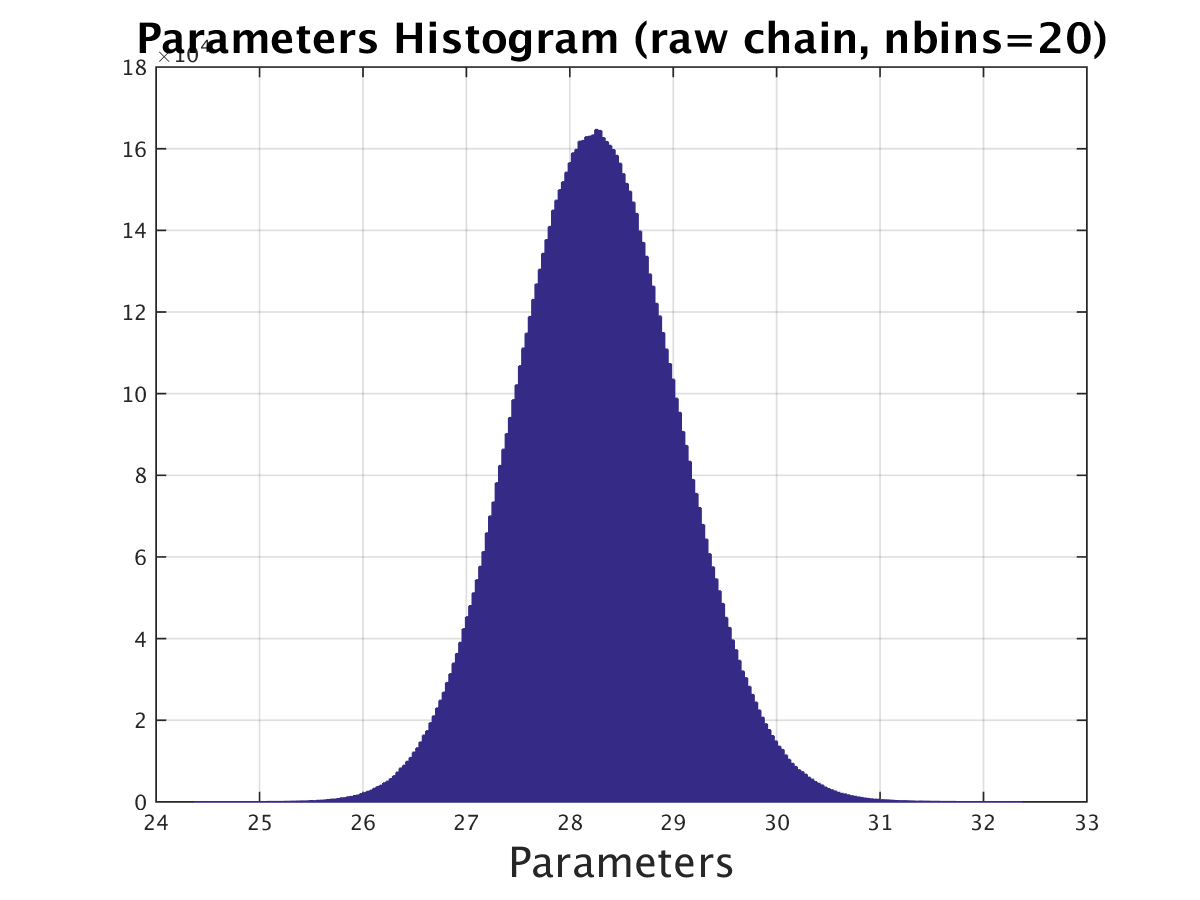
\includegraphics[scale=0.47]{model_1/simple_ip_hist_raw}
    }
\caption{MCMC raw chain and Histogram}
    \end{figure}
%
  \begin{figure}[H]
  \ContinuedFloat
  \centering
\subfloat[KDE \label{subfig-4:KDE}]{
        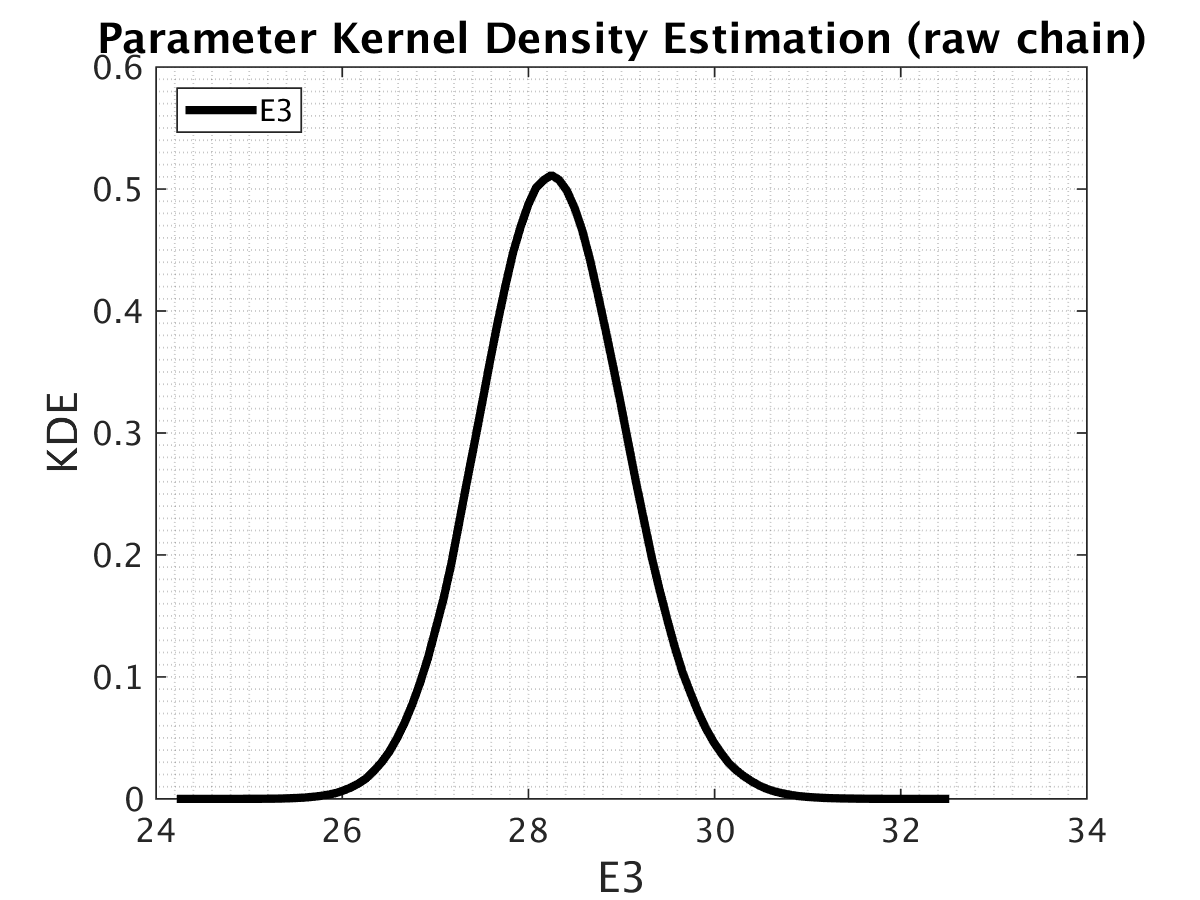
\includegraphics[scale=0.7]{model_1/simple_ip_kde_raw}
            }
\caption{ Parameter  kernel Density Estimation for $E_3$}
\end{figure}
%
%% \begin{figure}[H]
%%  \ContinuedFloat
%% \centering
%% \subfloat[LogLikelihood \label{subfig-5:Loglike}]{
%% 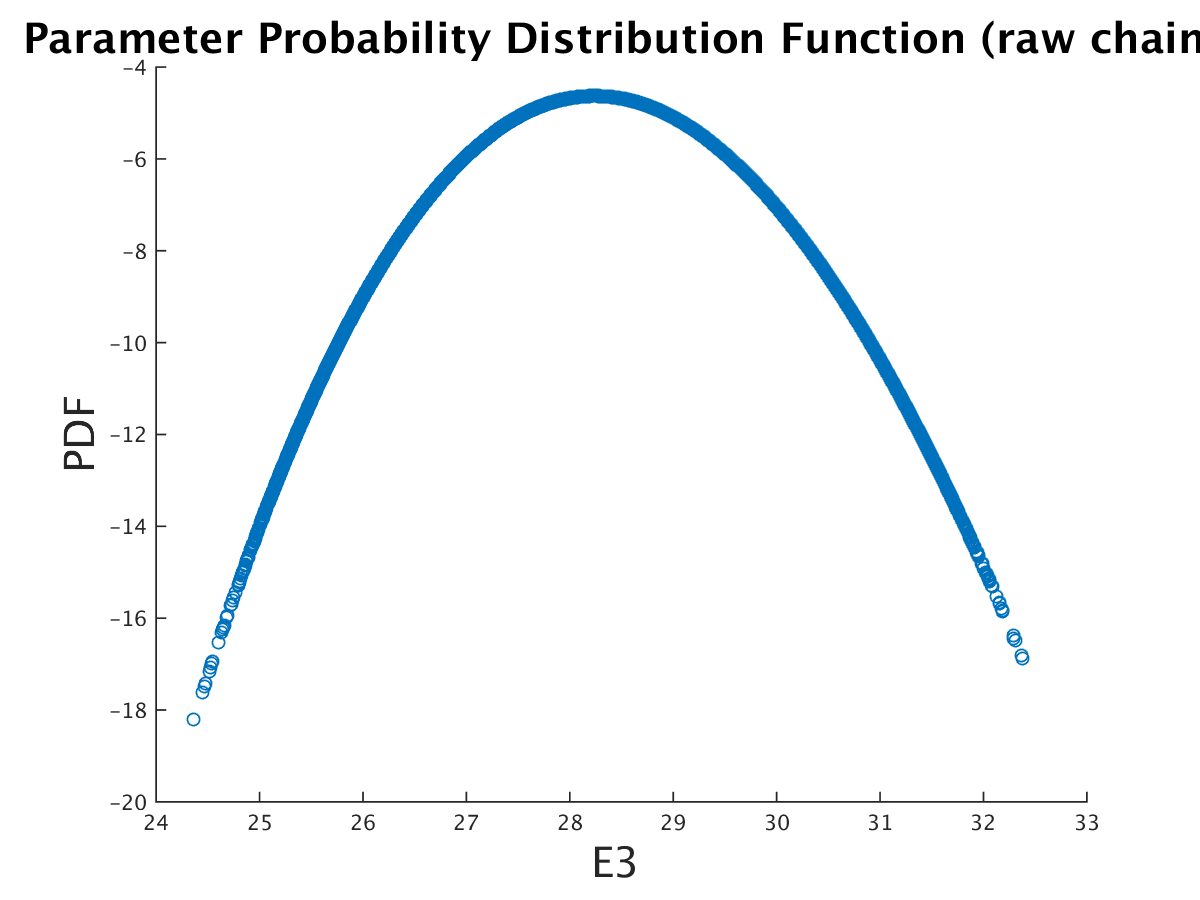
\includegraphics[scale=0.7]{model_1/ip_logLike_unified}
%%   }
%%     \caption{Results for sample size 1e7}
%% \end{figure}

\subsection{Convergence Study: Number of samples }

 In this section, we see the convergence of the probability distribution as we increase the raw chain sample size. The plot is done for surrogate size of 1000. In this analysis, raw chain size of $1e5$, $5e5$ , $1e6$, $5e6$ and $1e7$ is taken.

\begin{figure}[H]
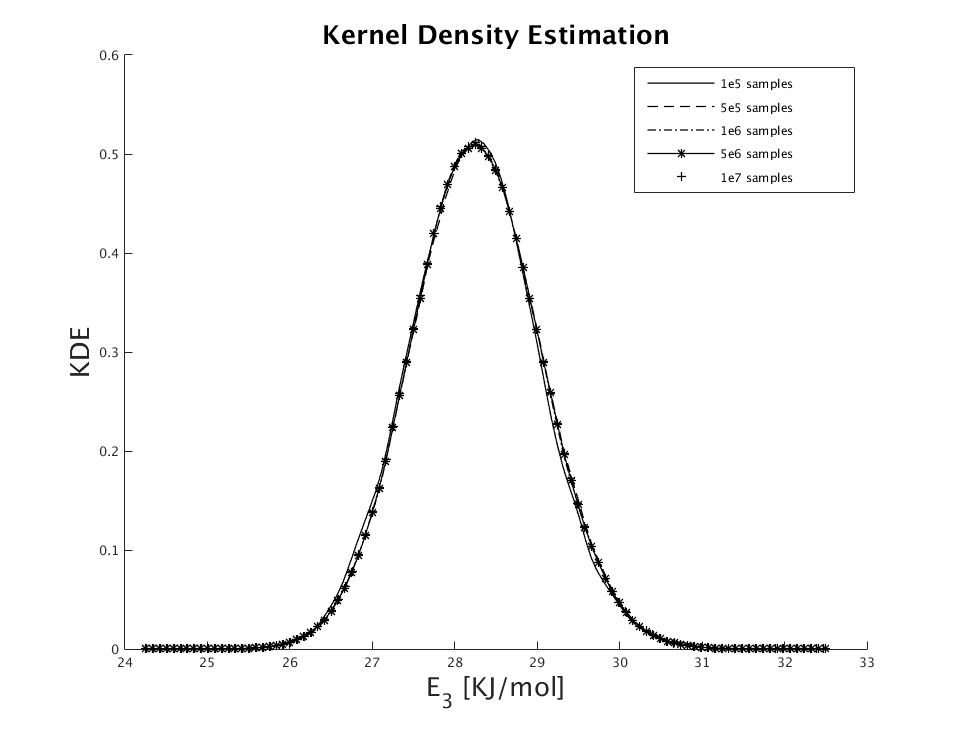
\includegraphics[scale = 0.35]{model_1/sample_conv}
    \caption{Convergence for surrogate size 1000}
\end{figure}


\subsection{Convergence Study: Surrogate }

 In this section, we see the convergence of the surrogate. As we increase the number of points in the surrogate, results should be close for different surrogate sizes. The plot is done for surrogate size of 100, 500 and 1000. In this analysis, raw sample chain size is $1e7$.

\begin{figure}[H]
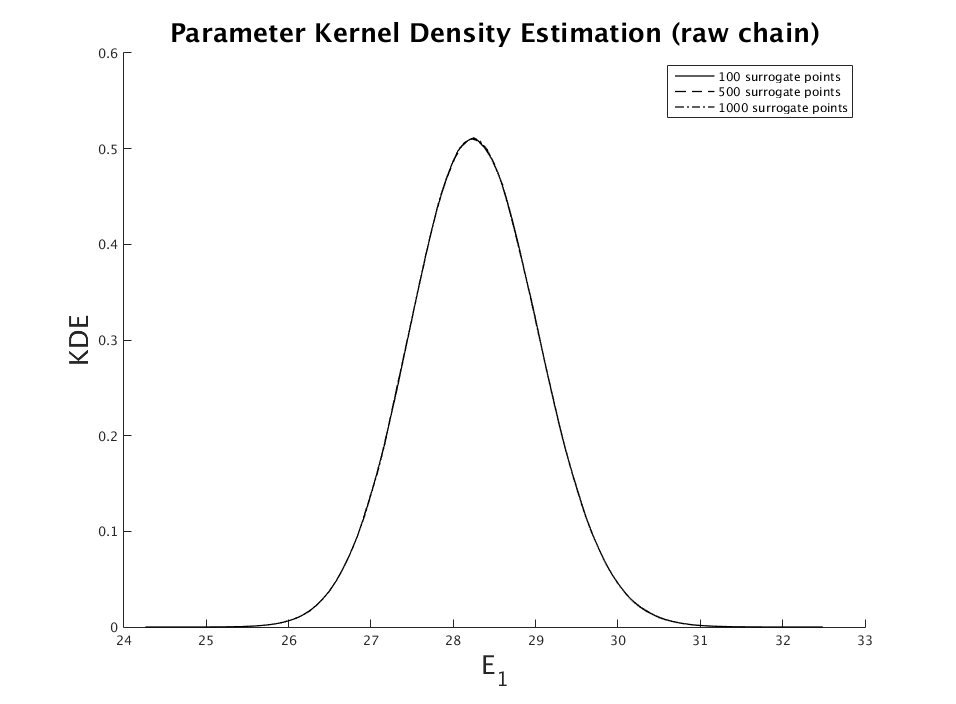
\includegraphics[scale=0.35]{model_1/conv_surrogate}
    \caption{Convergence for surrogate size 100, 500 and 1000}
\end{figure}


\subsection{Flamespeed Data fit}

 It is necessary to ensure that the samples of the parameter which we are drawing are fitting the flamespeed values of the experiment. In this section, we calculate the flamespeed for all the parameters drawn using the surrogate generated before. We have taken $1e7$ sample size and calculated flamespeed for different concentrations of ozone.

 \begin{figure}[H]
  \centering
   \subfloat[ Flame speed for 40 \% ozone \label{subfig-1:40}]{
        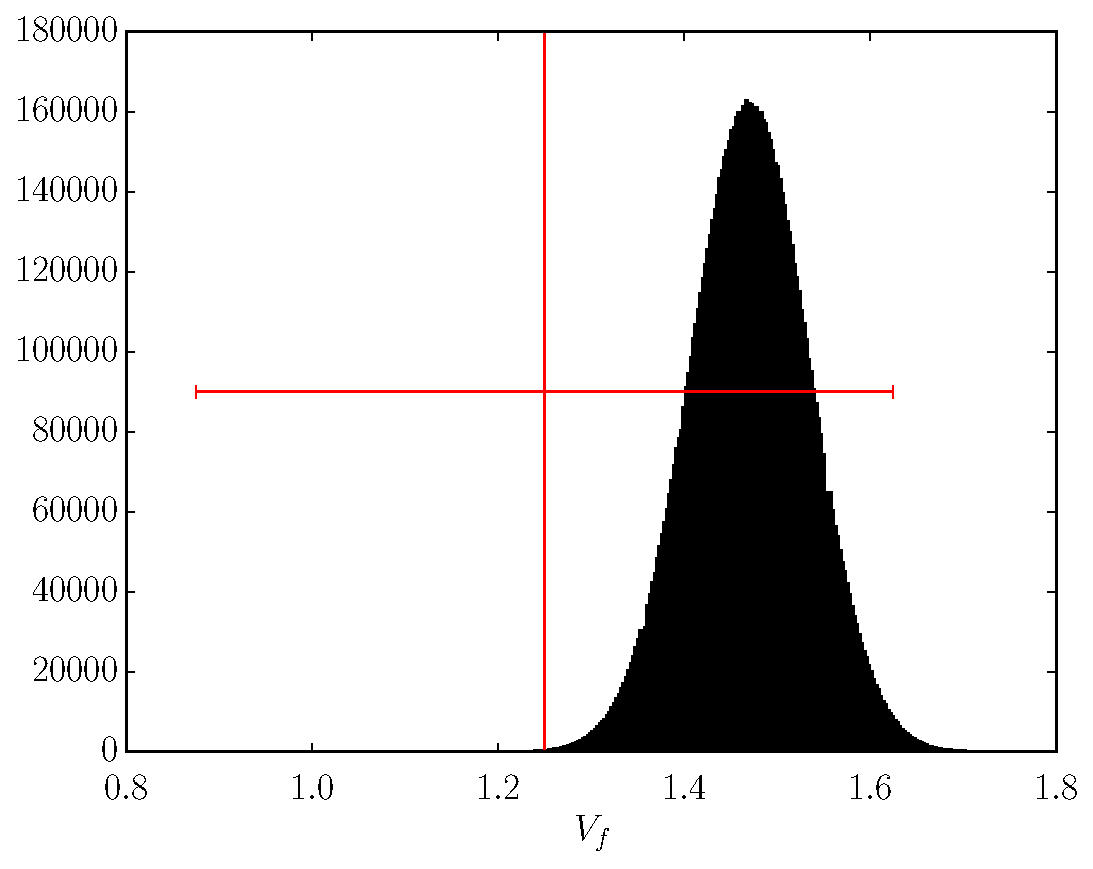
\includegraphics[scale=0.7]{model_1/flame_40.pdf}
       }
     \quad
\subfloat[Flame speed for 46 \% ozone \label{subfig-2:46}]{
        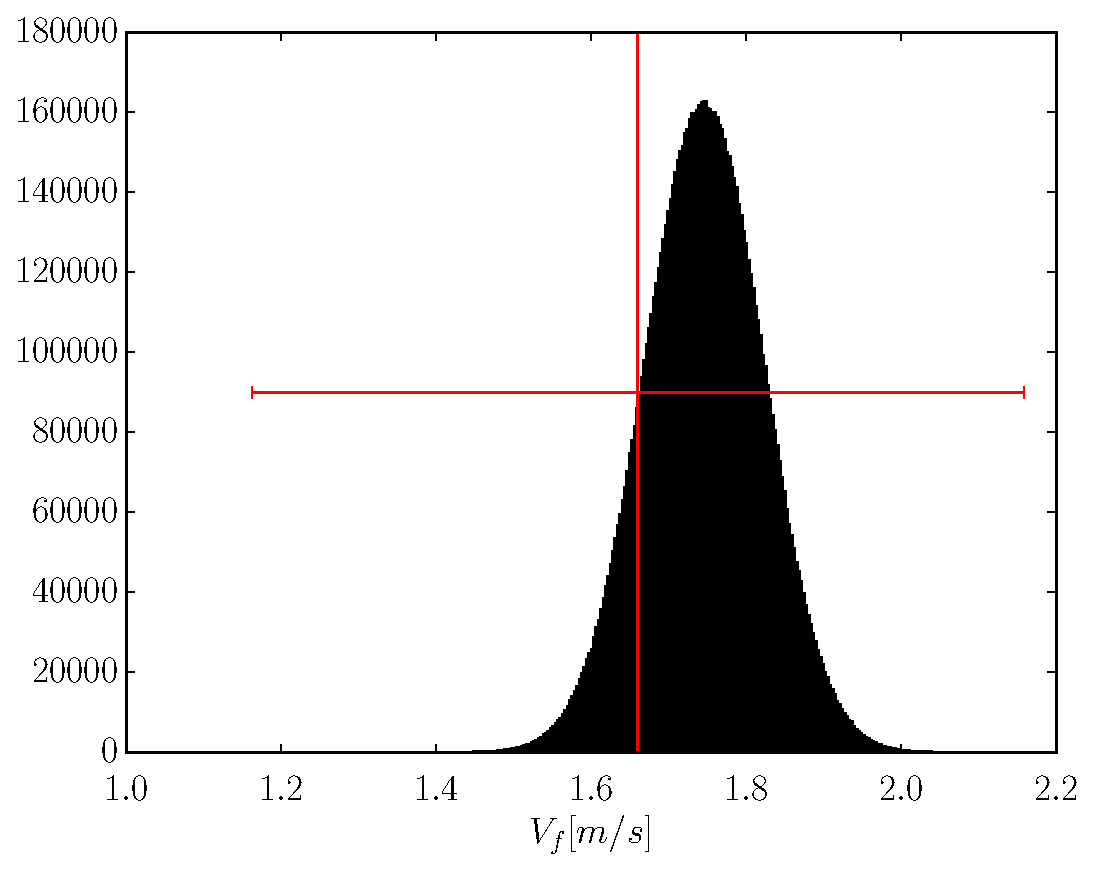
\includegraphics[scale=0.7]{model_1/flame_46.pdf}
            }
\end{figure}


 \begin{figure}[H]
  \ContinuedFloat
  \centering
   \subfloat[ Flame speed for 53 \% ozone \label{subfig-3:53}]{
        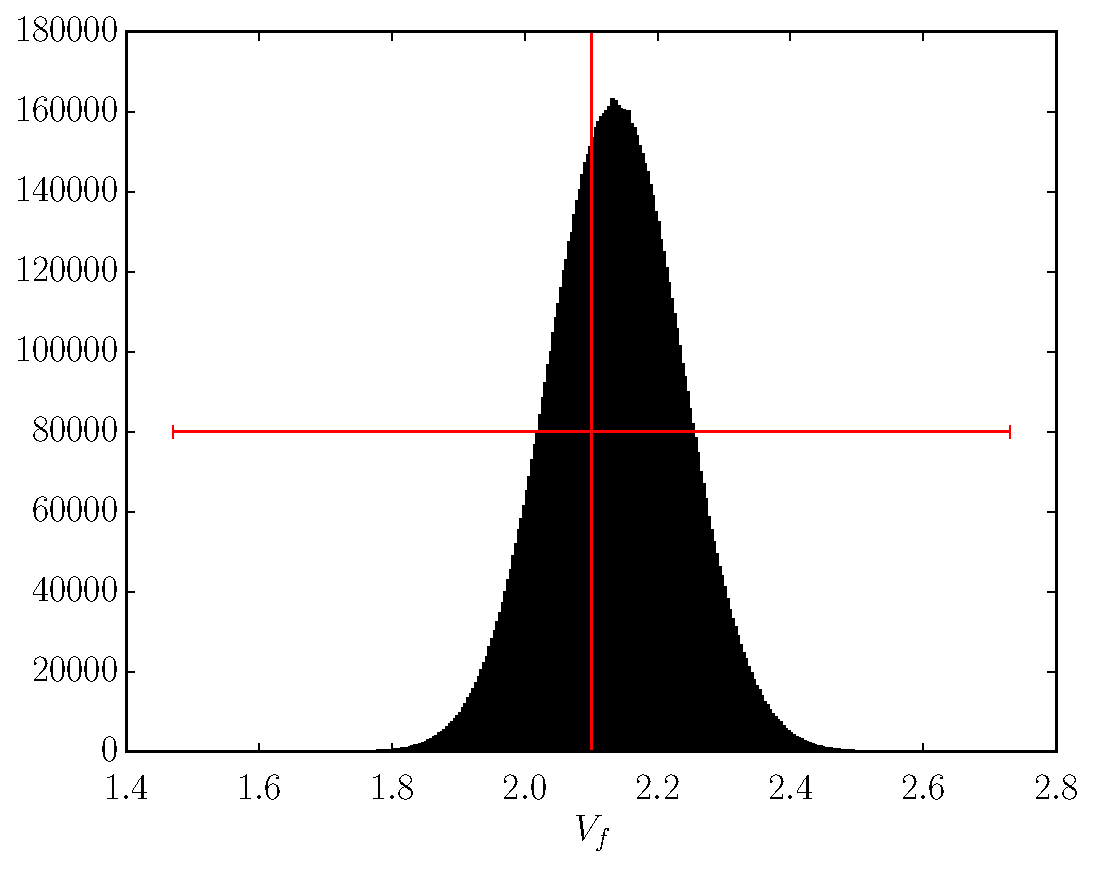
\includegraphics[scale=0.7]{model_1/flame_53.pdf}
       }
     \quad
\subfloat[Flame speed for 75 \% ozone \label{subfig-4:75}]{
        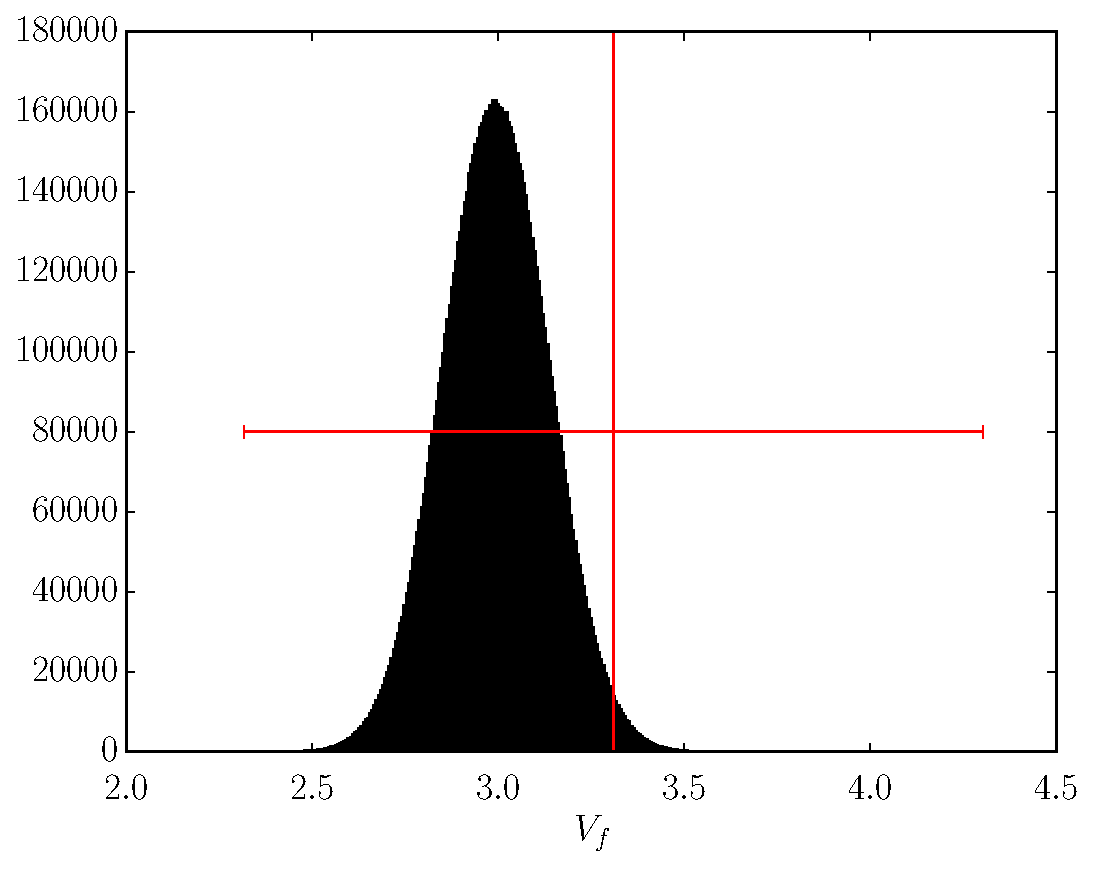
\includegraphics[scale=0.7]{model_1/flame_75.pdf}
            }
\end{figure}


 \begin{figure}[H]
  \ContinuedFloat
  \centering
   \subfloat[ Flame speed for 100 $\%$ ozone \label{subfig-5:100}]{
        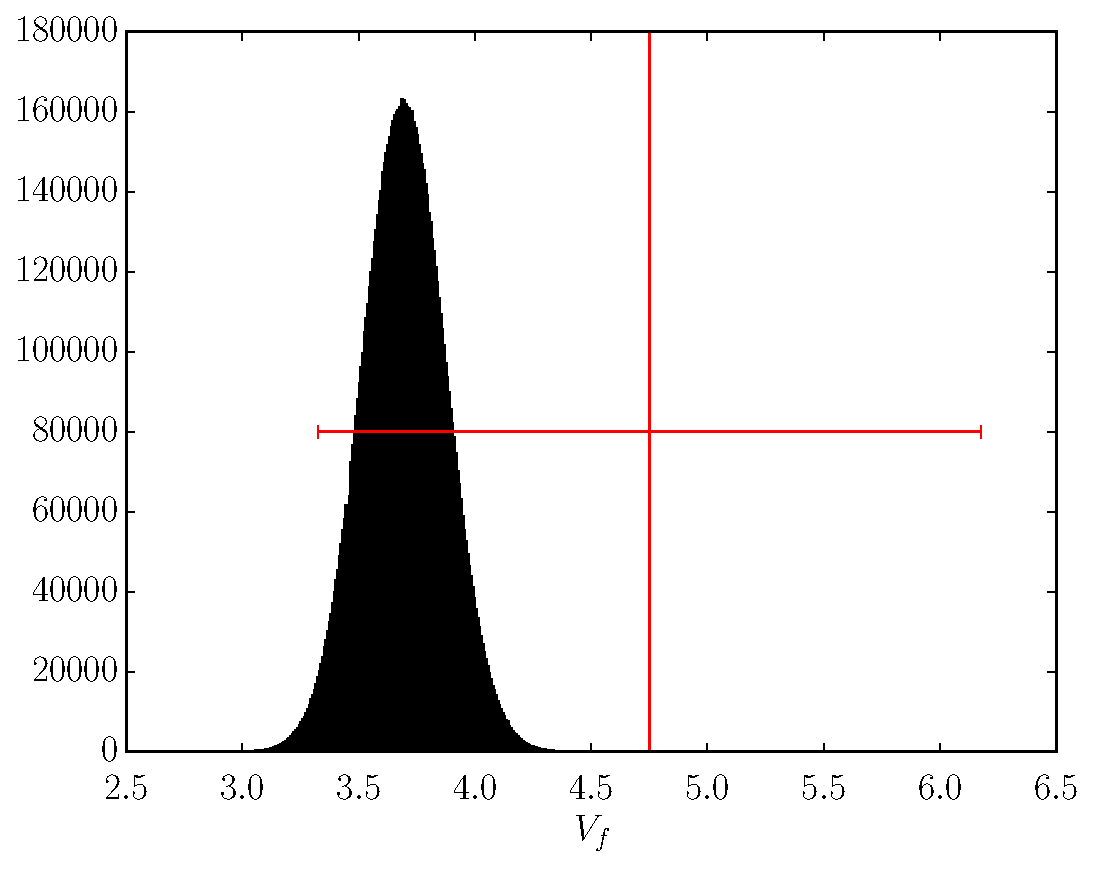
\includegraphics[scale=0.7]{model_1/flame_100.pdf}
       }
  \caption{Flamespeed Data fit}
\end{figure}



\subsection{Mean and Autocorrelation plots}

 In this section, we show the mean of the samples and autocorrelation plots . The mean plot shows the initial instability due to sum in period of MCMC and after that it remains constant. It shows us that we should be using at least more than these number of samples for our analysis. The last figure shows the histogram and the various parameters of the distribution are Mean:  28.3, Std. Dev.:  0.78, Skewness:  0.0666 and Kurtosis:  0.0352.


 \begin{figure}[H]
  \ContinuedFloat
  \centering
   \subfloat[ Mean  \label{subfig-1:mean}]{
        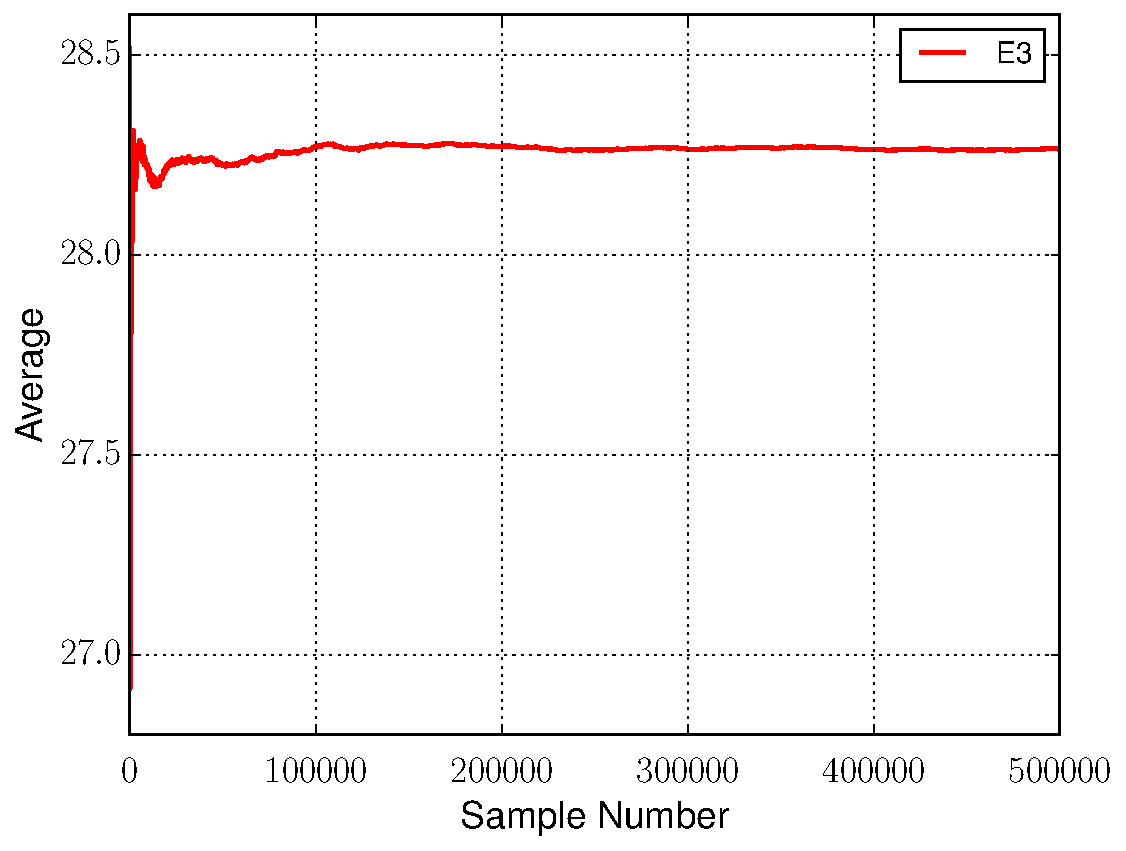
\includegraphics[scale=0.7]{model_1/M1_running_avg.pdf}
       }
     \quad
\subfloat[Autocorrelation  \label{subfig-2:auto}]{
        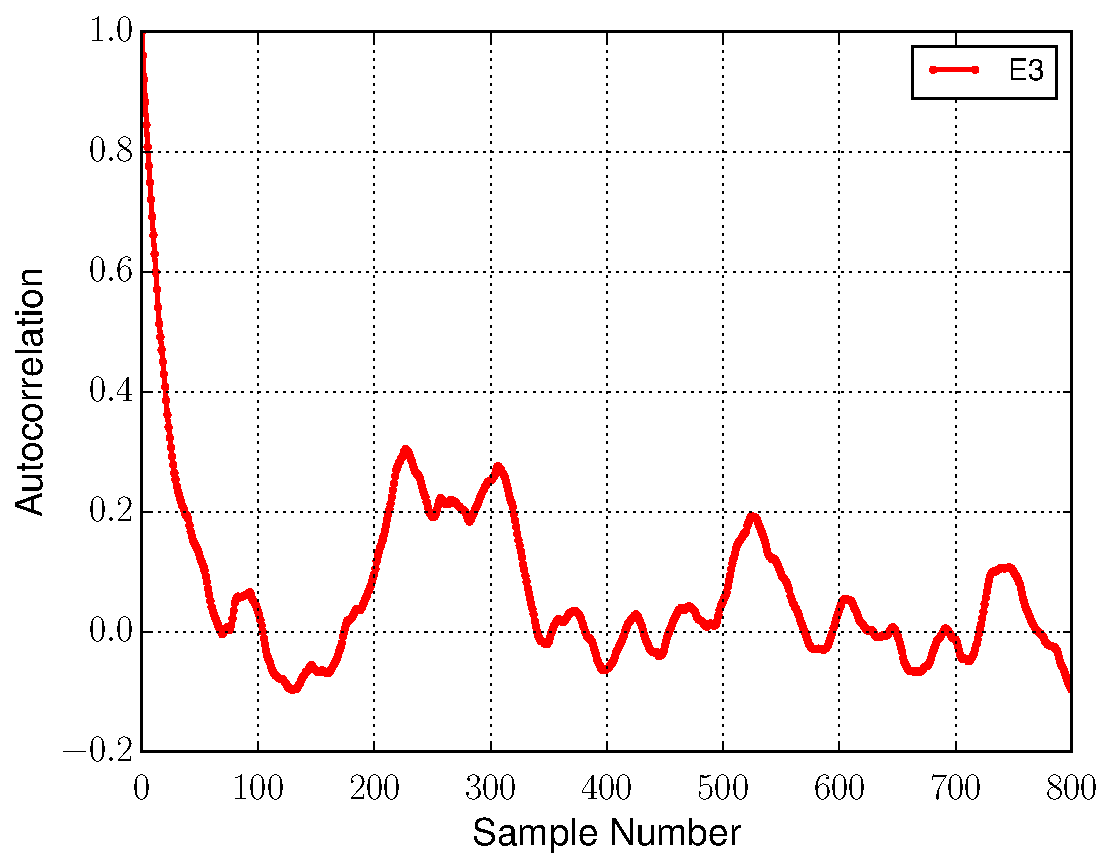
\includegraphics[scale=0.7]{model_1/M1_autocorr.pdf}
            }
            \caption{Mean and autocorrelation for sample size 1e7}
			\end{figure}
 \begin{figure}[H]
  \centering
\subfloat[ \label{subfig-2:auto}]{
        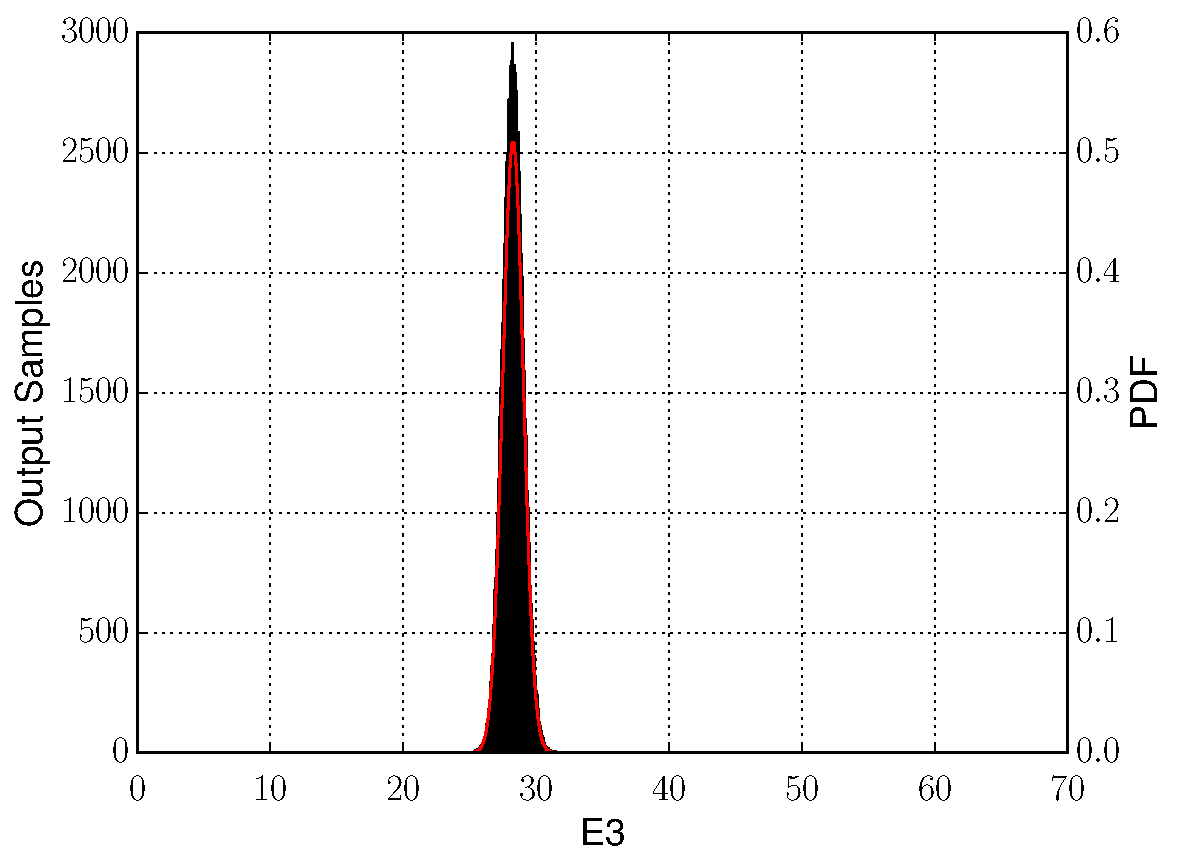
\includegraphics[scale=0.7]{model_1/E3.pdf}
            }
            \caption{Histogram}
\end{figure}
